\section{The Model for a Personalized HIV Treatment}
\label{sec:model}

In this section, we introduce a mathematical model that allows us to simulate the evolution of an HIV infection.
After further investigating this model and discussing the impact of antiretroviral drugs, the optimal control problem is formulated.

\subsection{The Dynamic Model}
\label{subsec:Model_DynModel}

Since HIV has first been simulated in the mid-90s, a wide variety of different models arose.
Initially, the latter attempted to investigate the HIV evolution by a set of linear \textit{ordinary differential 
equations} (ODEs). These however, are mere approximations of the realistic dynamics of viral pathogenesis and, hence only 
applicable for a short period of time, ranging in the orders of days.
HIV, treated or untreated, is a disease that extents over years and accurate and reliable long-term investigations 
require non-linear models \cite{adams2005hiv}.\newline
In addition hereto, the final model definition is determined by the choice of biological compartments and interactions 
that one wants to simulate.
Some models, for instance, differentiate between potential traget cells, usually including CD4+ T cells and macrophages \cite{perelson1993dynamics}.
Once a cell is infected, it can either remain in a latent state or actively reproduce new viral cells, causing different reaction of 
the patient’s immune system \cite{anderson1998complex}.\par

To optimize HAARTs, we require a model that does not only simulate the interaction between viral and immune cells but 
one that also considered the effect of the taken drugs.\newline
For this, we first have to review the working principle and impact of HAART.
% Finding such a model, demands for reviewing the working priciples of HAART.
Generally, this therapy is a combination of multiple classes of antiretroviral drugs, each fighting the virus in different ways.
Two of these are the so-called \textit{reverse transcriptase inhibitors} (RTIs) and the \textit{protease inhibitors} (PIs).
While the first aims at blocking the initial infection of target cells, the latter causes already infected cells to only produce 
immature virus.
Both these drugs, are solely designed for virus cells with a specific genome.
HIV, however, replicate in untreated persons at an exponentionally high rate, generating up to $10^{10}$ new free virus 
cells per day. Essential steps in this duplication are error-prone and hence, the probability of mutations is high.
The emerging cells have modified genomes, and the deployed drugs inhibt them less efficiently.
Thus, an appropriate model has to distiguish between drug-sensitive and resistant viruses \cite{rong2007emergence}.\par
According Rong et al. \cite{rong2007emergence}, a model that meets all our requirements, can be described by the following set 
of differential equations:

\begin{align}
    \begin{split}
        \dot{T}(t) &= \lambda - dT(t) - k_s (1 - \varepsilon_{RT}^s) V_s(t) T(t) - k_r (1 - \varepsilon_{RT}^r) V_r(t) T(t),\\
        \dot{T_s}(t) &= (1-u)k_s(1 - \varepsilon_{RT}^s)V_s(t)T(t) - \delta T_s(t),\\
        \dot{V_s}(t) &= N_s \delta (1 - \varepsilon_{PI}^s) T_s(t) - c V_s(t),\\
        \dot{T_r}(t) &= u k_s (1 - \varepsilon_{RT}^s) V_s(t) T(t) + k_r (1 - \varepsilon_{RT}^r) V_r(t) T(t) - \delta T_r(t),\\
        \dot{V_r}(t) &= N_r (1 - \varepsilon_{PI}^r) \delta T_r(t) - c V_r(t).
    \end{split}
    \label{equ:HIVmodel}
\end{align}

Here, $T(t)$ denotes the concentration of uninfected target T cells.
Generally, by index $s$ we denote the drug-sensitive strain whereas index $r$ marks the drug-resistant one.
% As discussed above, we are distiguishing between drug sensitive and resistant strains.
Thus, $T_s(t)$ is the concentration of cells that are infected by drug-sensitive viral cells $V_s(t)$.
$T_r(t)$ is the concentration of cells that are infected by drug-resistant viral cells $V_r(t)$.
Note, that all concentrations are given in $1/ml$.
The rate at which $T_s(t)$ cells become drug-resistant during the process of replication is given by the parameter $u$ ($0 \leq u < 1$).\newline
Further, $\lambda$ represents the birth rate of uninfected T cells per day, $d$ is their per capita daily death rate.
Apart from natural death, the T cell population is reduced by infection. $k_s$ and $k_r$ represent the constant rates at which 
uninfected cells are infected by drug sensitive and resistant virus, respectively.
At the same time, these rates are reduced by the use of RITs. The efficacy of the drug is given by the dimensionless 
parameters $\varepsilon_{RT}^{s}$ and $\varepsilon_{RT}^{r}$, both ranging between 0 and 1.
Since sensitive viruses are more susceptible to drugs, it is $\varepsilon_{RT}^{s} > \varepsilon_{RT}^{r}$.\newline
We assume that both kinds of infected cells, $T_s(t)$ and $T_r(t)$, burst and consequently die at the same daily rate $\delta$.
During bursting, a certain number of free virus cells are released. For sensitive virus cells, the number is denoted by $N_s$ 
while $N_r$ describes the same quantitiy in the drug-resistant case.
However, under the deployment of PIs, not all of the newly generated free virus cells are themselves capable of infecting healthy immune 
cells. This is encoded in the efficacy parameters $\varepsilon_{PI}^s$ and $\varepsilon_{PI}^r$. Again, it is $0 \leq \varepsilon_{PI}^s \leq 1$, 
$0 \leq \varepsilon_{PI}^r \leq 1$ and $\varepsilon_{PI}^s > \varepsilon_{PI}^r$.
Virus cell populations are only reduced by their daily clearance rate $c$.\newline
With the parameters $\varepsilon_{RT}$ and $\varepsilon_{PI}$, we describe the efficacy of the single antiretroviral drugs.
Summarizing these to the overall drug efficacy $\varepsilon = 1 - (1-\varepsilon_{RT})(1-\varepsilon_{PI})$ allows us to assess the efficacy of 
the combination therapy.
Hence, it is

\begin{align}
    \begin{split}
        \varepsilon_s &= 1 - (1-\varepsilon_{RT}^s)(1-\varepsilon_{PI}^s)\, ,\\
        \varepsilon_r &= 1 - (1-\varepsilon_{RT}^r)(1-\varepsilon_{PI}^r) \,\text{.}
    \end{split}
    \label{ref:epsilon_HAART}
\end{align}

In the following, we assume that the resistance level of the HIV mutants can be quantified by the parameter $\alpha\; (0 < \alpha < 1)$, 
which represents the reduction in drug efficacy by $\varepsilon_{s} = \alpha \varepsilon_{r}$.\newline
Descriptions and units of all parameters are summarized in table \ref{tab:init_parameters}.\par

\renewcommand{\arraystretch}{1.25}
\begin{table}
    \centering
    % \begin{tabular}{m{5em} m{10em} m{20em}}
        \begin{tabular}{ ccc }
        \hline
        \hline
        \multicolumn{3}{c}{\textit{Parameter definitions and values used in numerical simulation}} \\
        \hline
        % \rule{0pt}{10pt}
        Parameter & Value & Description\\[0.5ex]
        \hline
        $\lambda$   & $10^4\,\text{ml}^{-1}\text{day}^{-1}$ & Birth rate of uninfected cells\\
        $d$   & $0.01\,\text{day}^{-1}$  & Natural death rate of uninfected cells\\
        $k_s$   & $2.4 \times 10^{-8}\,\text{ml}\,\text{day}^{-1}$  & Infection rate of target cells by drug-sensitive virus\\
        $k_r$   & $2.0 \times 10^{-8}\,\text{ml}\,\text{day}^{-1}$  & Infection rate of target cells by drug-resistant virus\\
        $u$   & $3 \times 10^{-5}$  & Mutation rate from sensitive to resistant strain\\
        $\delta$   & $1\,\text{day}^{-1}$  & Death rate of infected cells\\
        $N_s$   & $3000$  & Burst size of drug-sensitive strain\\
        $N_r$   & $2000$ & Burst size of drug-resistant strain\\
        $c$   & $23\, \text{day}^{-1}$  & Clearance rate of free virus\\
        $\varepsilon_{RT}^{s}$   & varies & Efficacy of RTIs for sensitive strain\\
        $\varepsilon_{RT}^{r}$   & varies & Efficacy of RTIs for resistant strain\\
        $\varepsilon_{PI}^{s}$   & varies & Efficacy of PIs for sensitive strain\\
        $\varepsilon_{PI}^{r}$   & varies & Efficacy of PIs for resistant strain\\
        $\varepsilon_{s}$   & varies & Overall drug efficacy for sensitive strain\\
        $\varepsilon_{r}$   & varies & Overall drug efficacy for resistant strain\\
        $\alpha$   & varies & Resistance level of mutant strain\\
        \hline
        \hline
    \end{tabular}
    \caption{The tabel gives an overview about the model parameters, their definitions and physical units.
    The listed values, which are used for the numerical simulations to investigate the model, are based on a paper by Rong et al. \cite{rong2007emergence}.}
    \label{tab:init_parameters}
\end{table}

% The final objective is to derive model parameters from the clinical data of one patient, and hence explicitly tailor it to that person.
% However, before doing so, we are examining the model itself in more detail.
Before tailoring the above model \ref{equ:HIVmodel} to a specific patient, its dynamic and steady state behaviour is validated by comparing numerical results 
to clinical observations and findings from research.
In addition hereto, such simulations allow a deeper insight into the impact of antiretroviral drugs.
If not stated differently, parameters are taken from table \ref{tab:init_parameters}.\newline
Firstly, we consider a pretreatment situtaion.
A patient, who has been healthy until the very day of infection, has a CD4+ T cell count of $T(0) = 10^{6} \, \text{ml}^{-1}$.
If she or he is infected by a viral load of $V_s(0) = 10^{-6} \, \text{ml}^{-1}$, the untreated virus (i.e. $\varepsilon_s = \varepsilon_r = 0$) 
evolves within the first weeks as depicted in figure \ref{fig:untreated}.
Note, that although the transmitted pathogens could have already been mutated, it is assume that $V_r(0) = 0\, \text{ml}^{-1}$.
The further inital values are set $0$ \cite{perelson1993dynamics}.\newline
From figure \ref{fig:untreated} it can be seen, that the dynamic characteristics of the model coincide with the previously described stages
of an untreated HIV infection.
While in the first few weeks, the viral load increases strongly, the number of uninfected T cells collapses, resulting in often observed flu-like 
symptomes. 
% This phase is often accompanied by strong symptoms, resembling a flu.
Following this, the model shows how the state of clinical latency sets in.
Here, the viral loads as well as $T$ settle in a steady state.
Figure \ref{fig1c:viral_load} demonstrates that in the abscence of medication, the drug-sensitive strain dominates the infection throughout the 
considered time interval.

\begin{figure}
    \centering
    \begin{subfigure}[b]{0.475\textwidth}
        \centering
        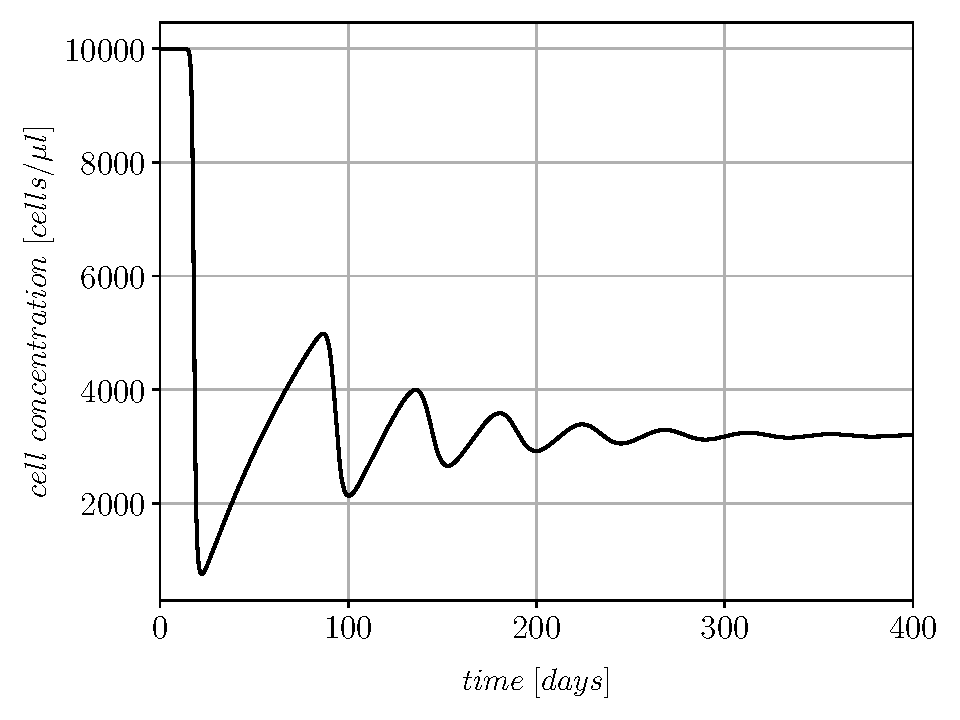
\includegraphics[width=\textwidth]{images/eRT_0_alpha_0/untreated_T.pdf}
        \caption[]%
        {{\small Uninfected CD4+ T cells}}    
        \label{fig1a:uninfected_T_cells}
    \end{subfigure}
    % \hfill
    % \begin{subfigure}[b]{0.3\textwidth}  
    %     \centering 
    %     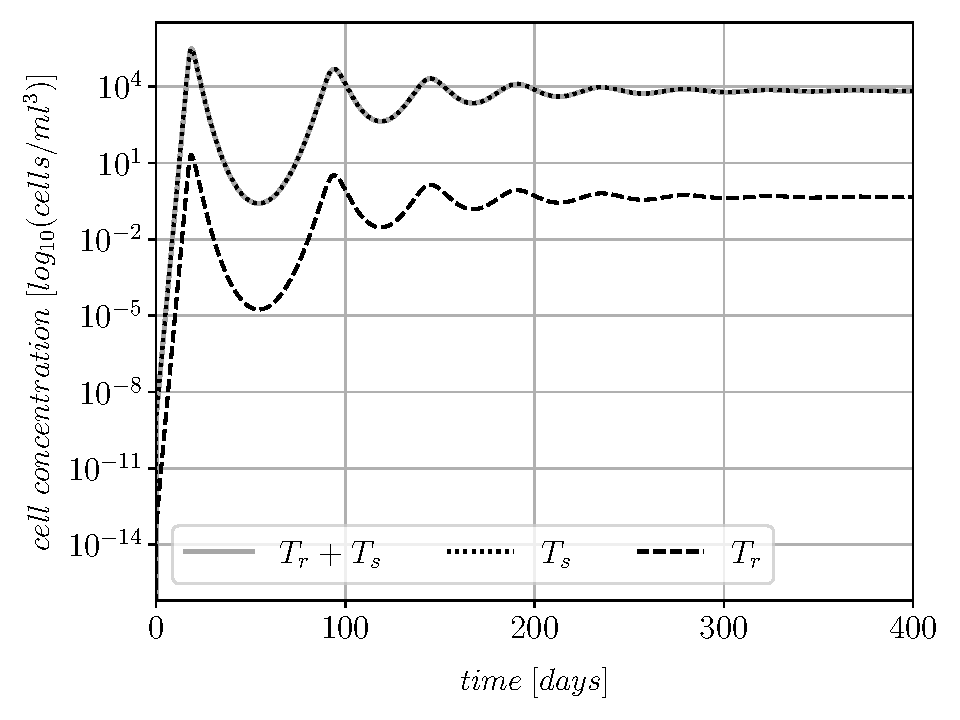
\includegraphics[width=\textwidth]{images/eRT_0_alpha_0/untreated_overview_infected_T.pdf}
    %     \caption[]%
    %     {{\small Infected CD4+ T cells}}    
    %     \label{fig1b:infected_T_cells}
    % \end{subfigure}
    % \vskip\baselineskip
    \begin{subfigure}[b]{0.475\textwidth}   
        \centering 
        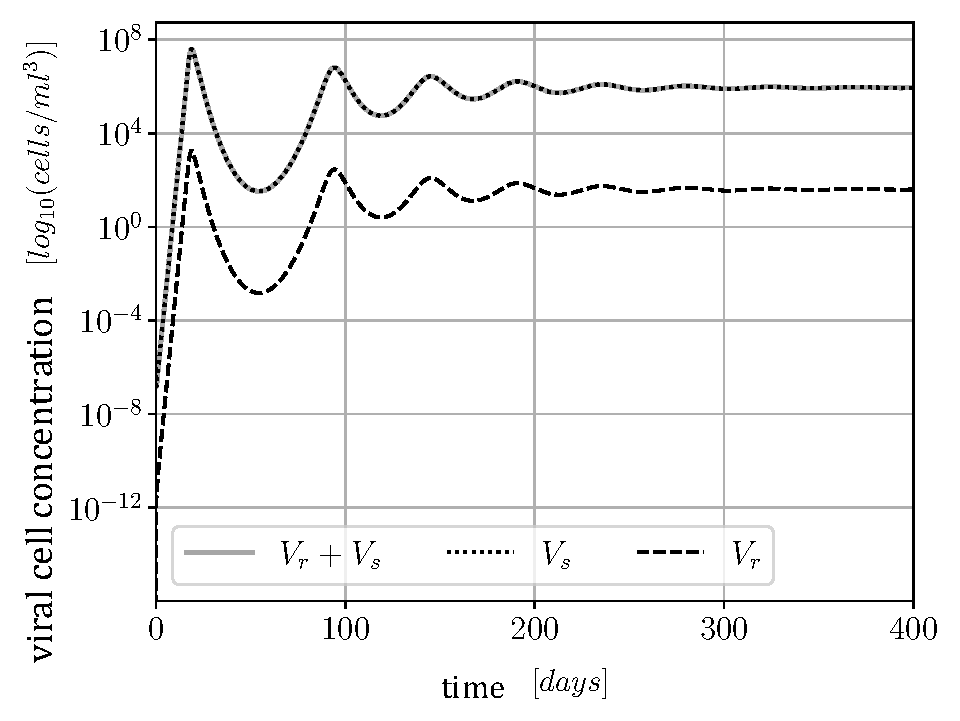
\includegraphics[width=\textwidth]{images/eRT_0_alpha_0/untreated_overview_V.pdf}
        \caption[]%
        {{\small Viral load}}    
        \label{fig1c:viral_load}
    \end{subfigure}
    \caption[]{Simulation of the pretreatment evolution of an initial HIV infection.
    For the inital state, the following values are assumed: $T(0) = 10^{6} \, \text{ml}^{-1}$, $T_s(0) = 0 \, \text{ml}^{-1}$, 
    $T_r(0) = 0 \, \text{ml}^{-1}$, $V_s(0) = 10^{-6} \, \text{ml}^{-1}$ and $V_r(0) = 0 \, \text{ml}^{-1}$ \cite{perelson1993dynamics}.}
    \label{fig:untreated}
\end{figure}

We assume that at this point of the disease, the infection is recognized and HAART is prescribed.
With a presumed low resistance level of $\alpha = 0.2$, the therapy is quantified by $\varepsilon_{RT}^{s} = 0.4$ and $\varepsilon_{PI}^{s} = \varepsilon_{PI}^{r} = 0$.
As initial values, the steady states of the pretreatment simualtion are chosen.\newline
The numerical results, given in figure \ref{fig2:treated_eRT_04_alpha_02}, show that indeed the therapy lowers the viral load and allows the 
number of uninfected immune cells to rise again.

\begin{figure}
    \centering
    \begin{subfigure}[b]{0.475\textwidth}
        \centering
        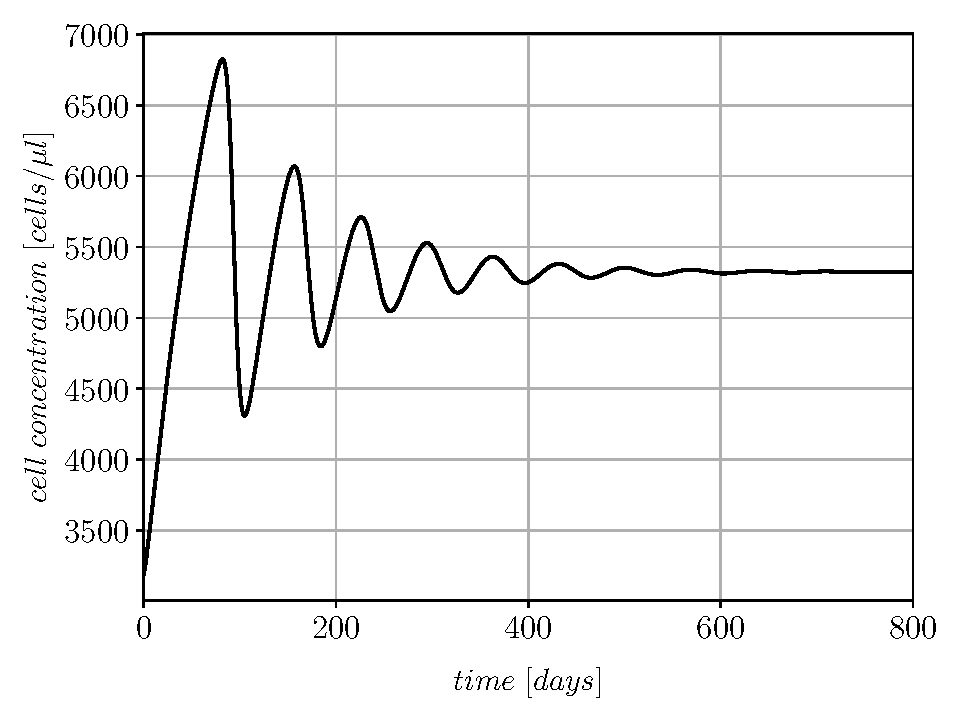
\includegraphics[width=\textwidth]{images/eRT_04_alpha_02/treated_T.pdf}
        \caption[]%
        {{\small Uninfected CD4+ T cells}}    
        \label{fig2a:uninfected_T_cells}
    \end{subfigure}
    % \hfill
    % \begin{subfigure}[b]{0.3\textwidth}  
    %     \centering 
    %     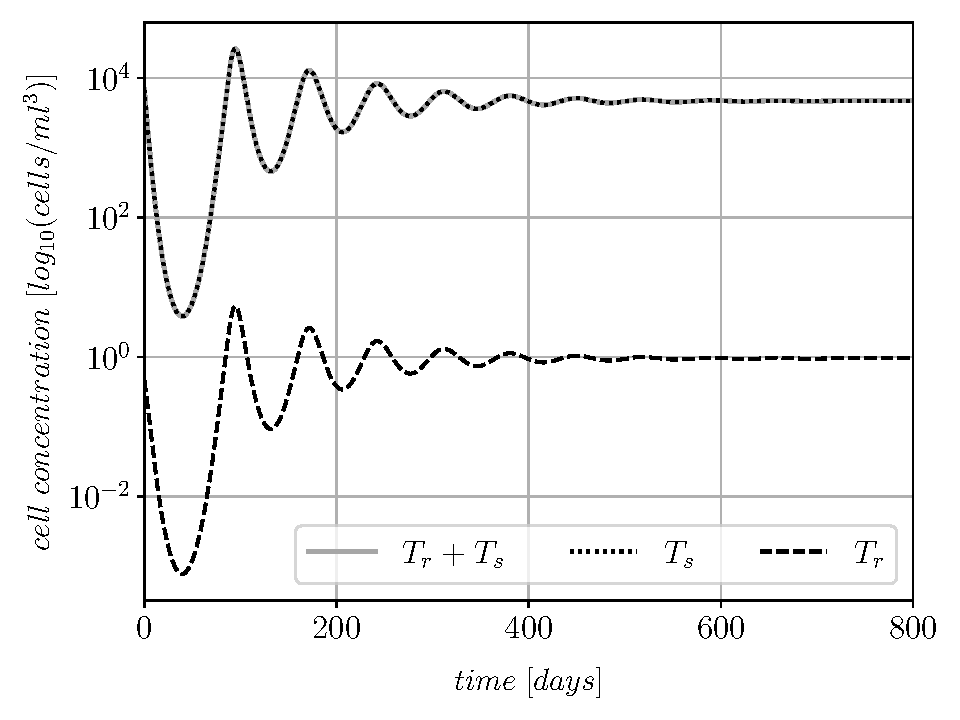
\includegraphics[width=\textwidth]{images/eRT_04_alpha_02/treated_overview_infected_T.pdf}
    %     \caption[]%
    %     {{\small Infected CD4+ T cells}}    
    %     \label{fig2b:infected_T_cells}
    % \end{subfigure}
    % \vskip\baselineskip
    \begin{subfigure}[b]{0.475\textwidth}   
        \centering 
        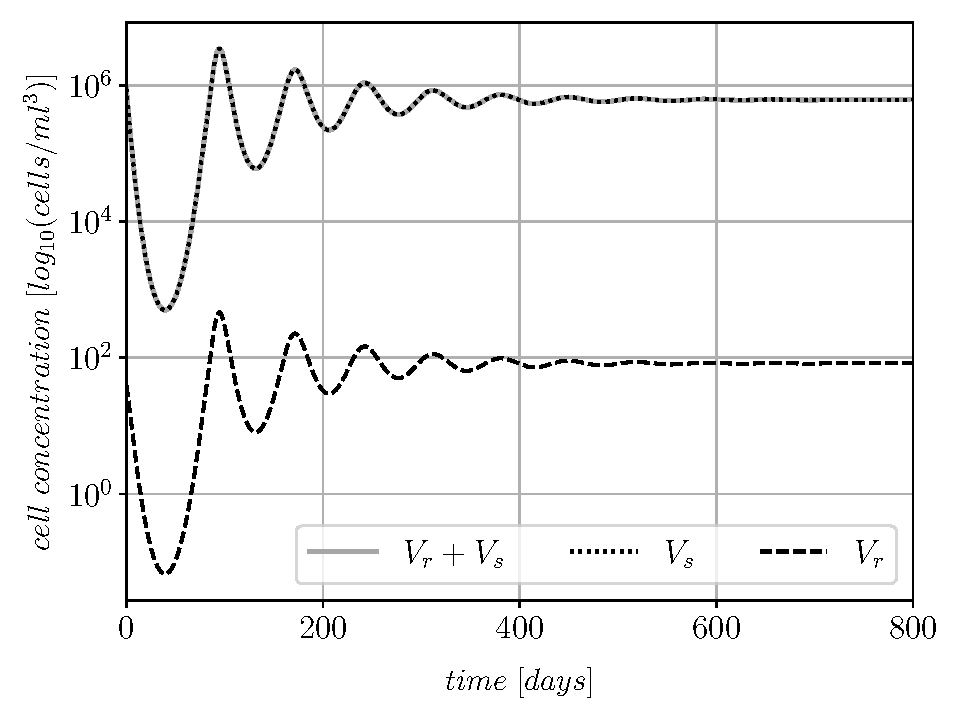
\includegraphics[width=\textwidth]{images/eRT_04_alpha_02/treated_overview_V.pdf}
        \caption[]%
        {{\small Viral load}}    
        \label{fig2c:viral_load}
    \end{subfigure}
    \caption[]{Simulation of the evolution of an HIV infection under HAART.
    It is $\varepsilon_{RT}^s = 0.4$, $\varepsilon_{RT}^r = \alpha \varepsilon_{RT}^s$ with $\alpha = 0.2$ and 
    $\varepsilon_{PI}^s = \varepsilon_{PI}^r = 0$.
    The steady states of the preceding pretreatment simulation are used as initial values, i.e. $T(0) = 3.19 \times 10^{5} \, \text{ml}^{-1}$, 
    $T_s(0) = 6.81 \times 10^{3} \, \text{ml}^{-1}$, $T_r(0) = 0.46 \, \text{ml}^{-1}$, $V_s(0) = 8.88 \times 10^{5} \, \text{ml}^{-1}$ 
    and $V_r(0) = 39.95 \, \text{ml}^{-1}$ \cite{perelson1993dynamics}.}
    \label{fig2:treated_eRT_04_alpha_02}
\end{figure}

An essential feature of the model is the development of the steady states as a function of medication efficacy of the drug-sensitive strain.
This is demonstrated in figure \ref{fig3:evolution_over_epsilon}, where the CD4+ T cell and viral count are plotted over $\varepsilon_s$.
From diagram \ref{fig3a:uninfected_T_cells}, it can be seen that for low values of $\varepsilon_s$, HAART achieve an increase in the 
number of uninfected target cells.
However, above a certain point, this growth saturates and the concentration remains on a constantly high level.
We denote this point of maximal efficacy by $\varepsilon_{s,max}$. 
For the given set of model parameters, its value is $\varepsilon_{s,max} \approx 0.5$.
A similar behaviour can be observed on the virus side, shown in figure \ref{fig3c:viral_load}.
In the lower $\varepsilon_s$ regime, the total virus count behaves reciprocally proportional to drug efficacy.
For $\varepsilon_{s,max} \leq \varepsilon_{s}$ this reduction halts after a large drop and the number of free virus settles in a steady state.\newline
% Obviously, further increasing the dose or potency of the drug does not lead to an improvement.\newline
An explanation for this behaviour can be found by investigating the evolution of the viral load more closely.
While the inital success of the therapy is based on pushing the number of $V_s$ beneath the threshold of detectability, 
the point of saturation sets in when the concentration of the drug-resistant strain erraticly increases.
The following consistency of the infection arises from two factors.
Firstly, due to the low level of $V_s$ no new mutations emerge.
Secondly, RTIs inhibit novel infections of the target cells and hence, the number of drug-resistant virus remains on a stable level.
Note, that due to the definition $\varepsilon_{RT}^r = \alpha \varepsilon_{RT}^s$, antiretroviral medications are not in- but only less 
efficient in attacking drug-resistant viruses (as long as $\alpha > 0$).\newline
The quintessence hereof is, that above a certain value $\varepsilon_{s,max}$, simply increasing dose or potency of antiretroviral drugs does not automatically 
result in an improvement of the therapy but only in an enhancement of their side effects.
At the same time, this turning point depends on the model parameters, i.e. on each patient individually.
This finding emphasises the necessity to personalize the model.

\begin{figure}
    \centering
    \begin{subfigure}[b]{0.475\textwidth}
        \centering
        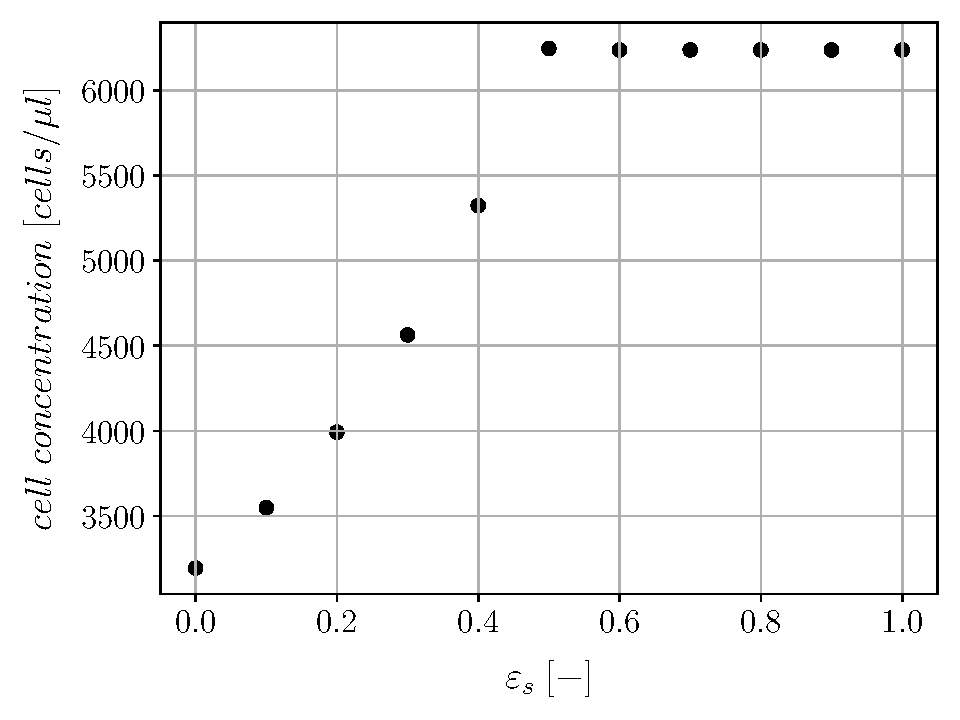
\includegraphics[width=\textwidth]{images/evolution_over_epsilon/treated_T.pdf}
        \caption[]%
        {{\small Uninfected CD4+ T cells}}    
        \label{fig3a:uninfected_T_cells}
    \end{subfigure}
    % \hfill
    % \begin{subfigure}[b]{0.3\textwidth}  
    %     \centering 
    %     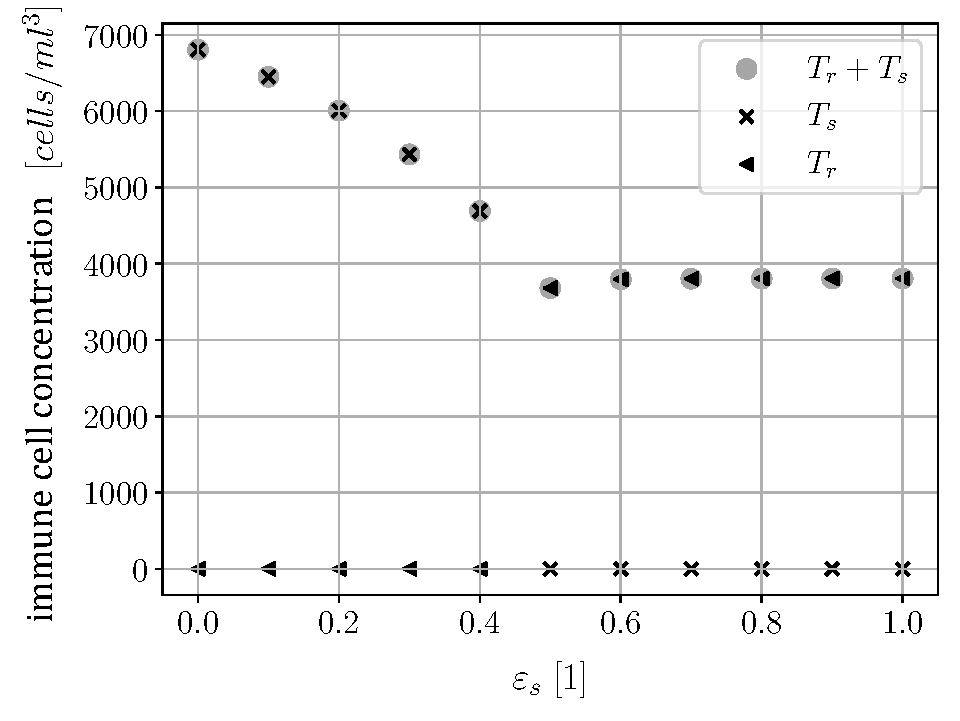
\includegraphics[width=\textwidth]{images/evolution_over_epsilon/treated_overview_infected_T.pdf}
    %     \caption[]%
    %     {{\small Infected CD4+ T cells}}    
    %     \label{fig3b:infected_T_cells}
    % \end{subfigure}
    % \vskip\baselineskip
    \begin{subfigure}[b]{0.475\textwidth}   
        \centering 
        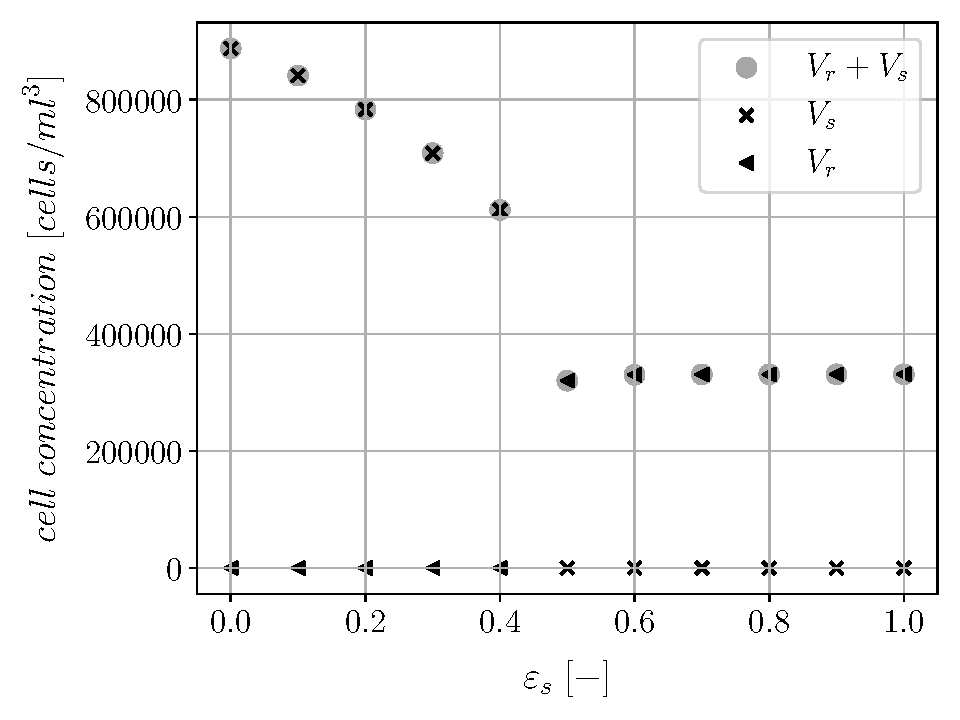
\includegraphics[width=\textwidth]{images/evolution_over_epsilon/treated_overview_V.pdf}
        \caption[]%
        {{\small Viral load}}    
        \label{fig3c:viral_load}
    \end{subfigure}
    \caption[]{The above diagrams show the evolutoin of the HIV infection in dependency of the drug efficacy parameter $\varepsilon_s$.
    In the considered case, it is $\varepsilon_{PI}^s =0$, $\varepsilon_{RT}^s = 0.4$ and $\alpha = 0.2$.
    Hence, the simulations basically demonstrate the impact of RTIs.}
    \label{fig3:evolution_over_epsilon}
\end{figure}

\subsection{The Optimal Control Problem}
\label{subsec:Model_OptControl}

An optimal therapy is one, that maximizes the level of CD4+ T cells while deploying as little drugs as possible.
Here, we assume that more and stronger drugs, i.e. higher $\varepsilon_s$ and $\varepsilon_r$, are associated with heavier 
side effects. 
Further, as shown in the preceding subsection \ref{subsec:Model_DynModel}, above a certain threshold efficacy $\varepsilon_{s,max}$, the effects of 
HAART saturate.\newline
From mathematical point of view, finding an ideal therapy can be formulated as an optimal control problem.
For this, we quantifiy the cost of HAART in the time interval $[t_0,t_1]$, by the functional

\begin{align}
    J(\mathbf{\varepsilon}) = \int_{t_0}^{t_1} \left(T^2(t) - A_1 \varepsilon_{s}^2 - A_2 \varepsilon_{r}^2\right) dt
    \label{equ:cost_function}
\end{align}

where $\mathbf{\varepsilon} = (\varepsilon_s, \varepsilon_r)^T \in [0,1]^2$ are the control parameters and $A_1$ and $A_2$ their 
weight constants \cite{adams2005hiv,wu2010game}.
The second term represents the cost of the drug treatment, which is to be minimized.
Hence, we seek an optimal control $\mathbf{\varepsilon}_{opt}$, such that

\begin{align}
    \mathbf{\varepsilon}_{opt} = \underset{\mathbf{\varepsilon} \in [0,1]^2}{\arg\max}\, (J(\mathbf{\varepsilon}_{opt})) \text{.}
    \label{equ:opti_control}
\end{align}
